\documentclass[a4paper, 12pt, twoside]{report}

\usepackage{physics, amsmath, amsfonts, siunitx}
\usepackage{tcolorbox}
\usepackage{enumitem}
\usepackage{hyperref}
\usepackage{graphicx}
\graphicspath{ {./ch1} }
\hypersetup{
        colorlinks=true,
                linkcolor=black,
                urlcolor=blue,
}

\usepackage{geometry}
\geometry{
        top=2cm,
                bottom=2cm,
                left=2cm,
                right=3cm,
                headheight=17pt,
                includeheadfoot,
}

\usepackage{fancyhdr, lastpage}
\pagestyle{fancy}
\fancyhf{}
\lhead{Mettere icona GitHub}
\rhead{ Relatività Ristretta }
\cfoot{Pagina \thepage\ di \pageref{LastPage}}
\renewcommand{\headrulewidth}{1.0pt}

\usepackage{etoolbox}
\patchcmd{\chapter}{\thispagestyle{plain}}{\thispagestyle{fancy}}{}{}

\title{Fisica nucleare e subnucleare}
\author{Pietro Garofalo}
\date{\today}


\begin{document}

\maketitle
\newpage
\tableofcontents
\chapter{Le trasformazioni di Lorentz }
In relatività le trasformazioni di Galileo sono sostituite dalle trasformazioni di Lorentz, prima di vederle nel dettaglio bisogna ricordarsi 
che le grandezze che ci interessano non sono più i semplici vettori ma i \textbf{ quadrivettori contravarianti } che definiamo nel seguente modo :
\begin{center}
        
        $ \vectorbold{X^{\mu}} = \begin{pmatrix} ct\\ \va{x} \end{pmatrix} $

\end{center}
Tale notazione evidenzia come i quadrivettori siano divisi in una parte temporale ( la prima componente ) e componenti spaziali ( vettore tridimensionale ), 
tali quaterne di valori trasformano, nel passaggio da un sistema di riferimento ad un altro, tramite le trasformazioni di Lorentz. \\
La metrica dei quadrivettori non è la metrica Euclidea bensì quella di \textbf{Minkowski}, se definiamo infatti due quadrivettori 
\begin{align*}
        \vectorbold{A^{\mu}} = \begin{pmatrix} a_0\\a_1\\a_2\\a_3\end{pmatrix}
        \
        \vectorbold{B^{\mu}} = \begin{pmatrix} b_0\\b_1\\b_2\\b_3\end{pmatrix}
\end{align*}
Allora il prodotto fra i due si definisce come :
\begin{align*}
        \vectorbold{A^{\mu}}\vdot\vectorbold{B_{\mu}} = a_0b_0 - a_1b_1 - a_2b_2 - a_3b_3
\end{align*}
dove $\vectorbold{B_{\mu}}$ non è altro che il \textbf{quadrivettore covariante} ossia il quadrivettore contravariante ma con il segno della parte spaziale opposto .\\
D'ora in avanti indicheremo $\vectorbold{X} \equiv \vb{X^{\mu}} $.
\newpage

\section{Trasformazione delle coordinate}
Supponiamo di avere un sistema di riferimento $\mathbb O$ fermo ( sistema del laboratorio ) e un sistema $\mathbb O^{'} $ in movimento 
con velocità V come in figura.\\

\begin{figure}[!h]
        \centering 
        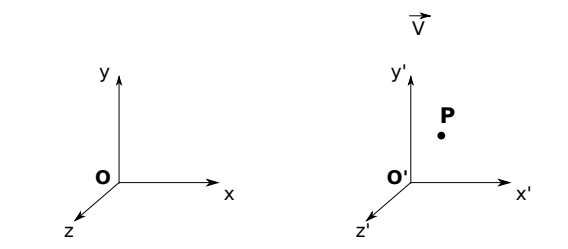
\includegraphics[scale=0.8]{SistemaRiferimento}
        \caption{Sistemi di riferimento}
\end{figure}
Indichiamo con $\vb{X}$ il quadrivettore posizione del punto \textbf{P} rispetto a $\mathbb O$ e $\vb{X^\prime}$ rispetto a $\mathbb O^\prime$, le coordinate di 
$\vb{X^\prime}$ si trovano rispetto alle coordinate misurate in $\mathbb O^\prime$ nel seguente modo : 
\begin{align*}
        \vectorbold{X^\prime} = \vb{\Lambda^{\mu}_{\nu}} \vb{X} 
\end{align*} 
dove $\vb{\Lambda^{\mu}_{\nu}}$ rappresenta la matrice della trasformazione di Lorentz lungo asse x data da : 
\begin{align*}
        \vb{\Lambda^{\mu}_{\nu}} = \begin{pmatrix} \gamma & -\gamma\beta & 0 & 0 \\ -\gamma\beta & \gamma & 0 & 0 \\ 0 & 0 & 1 & 0 \\ 0 & 0 & 0 & 1 \end{pmatrix} \tag*{$\beta = \frac{V}{c}$ \ $\gamma = \frac{1}{\sqrt{1-\beta^2}}$}
\end{align*}
si ottiene quindi il seguente sistema : 
\begin{equation*}
\left\{ \begin{aligned}
        ct^{\prime}&=\gamma(ct - \beta x) \\
        x^{\prime}&= \gamma( x - ct\beta ) \\
        y^{\prime}&= y \\
        z^{\prime} &= z
  \end{aligned}
  \right.
\end{equation*}
\begin{tcolorbox}[colback=red!5!white,colframe=red!50!black,title=ATTENZIONE !]
Se il cambio di sistema di riferimento si fa dal sistema in moto al sistema di riferimento del laboratorio allora $\beta$ cambia di segno 
\end{tcolorbox}
\newpage
\section{Trasformazione delle velocità}
Per capire bene le trasformazioni delle velocità conviene vedere un esercizio.\\
\begin{center}\textbf{Esercizio  }\end{center} 
Un uomo in automobile viaggia ad una velocità di $\frac{3}{4}c$, viene inseguito da un'altra automobile che va alla velocità di $\frac{1}{2}c$ 
la quale spara un proiettile che va alla velocità di $\frac{1}{3}c$.
Il proiettile raggiunge l'auto ? \\
\begin{center}\textbf{Soluzione}\end{center}
La questione è tutta basata sulle trasformazioni delle velocità in relatività, le troveremo tramite le trasformazioni di Lorentz viste prima, 
un commento prima di trovarle : 
\\
\begin{tcolorbox}[colback=red!5!white,colframe=red!50!black,title=ATTENZIONE !]
Bisogna capire bene i sistemi di riferimento, nel nostro caso stiamo osservando le macchine che corrono, noi siamo il laboratorio ( sistema fermo )
il problema è che la velocità del proiettile è calcolata nel sistema di riferimento in moto ( ossia la macchina che spara ), il gioco è tutto quì : 
trasformare la velocità del proiettile dal sistema di riferimento in moto a quello del laboratorio . 
\end{tcolorbox}
Partiamo dalla trasformazione di Lorentz per la posizione, come al solito identifichiamo con $x^{\prime}$ le coordinate del sistema di riferimento in moto : 
\begin{equation*}
\left\{ \begin{aligned}
                ct&=\gamma(ct^{\prime} + \beta x^{\prime}) \\
        x&= \gamma( x^{\prime} + ct\beta ) \\
        y&= y^{\prime} \\
        z&= z^{\prime}
  \end{aligned}
  \right.
\end{equation*}
Notare come c'è il cambio di segno dovuto al fatto che passiamo da sistema in moto a quello del laboratorio. \\
Passiamo ora agli infinitesimi : 
\begin{equation*}
        \left\{ \begin{aligned}
                        c\dd{t} &= \gamma c\dd{t^{\prime}} + \beta\gamma\dd{x^{\prime}} \\
                        \dd{x} &= \gamma\dd{x^{\prime}} + c\gamma\beta\dd{t^{\prime}} \\
                        \dd{y} &= \dd{y^{\prime}} \\
                        \dd{z} &= \dd{z^{\prime}} \\
                \end{aligned}
                \right.
\end{equation*}
Dividiamo ora ciascuna componente per $\dd{t}$ la cui espressione l'abbiamo ricavata sopra, dividiamo poi numeratore e denominatore per $\dd{t^{\prime}}$, sostiuiamo $ \frac{\dd{x^{\prime}}}{\dd{t^{\prime}}} \equiv \dd{v^{\prime}_{x}} $ eccetera, inoltre $\beta \equiv \frac{V}{c}$ 
dove V è la velocità del proiettile nel sistema in moto, si ottiene : 
\newpage
\begin{equation*}
        \left\{ \begin{aligned}
                        \frac{\dd{x}}{\dd{t}} &\equiv v_{x}&= \frac{\gamma v^{\prime}_{x} + \gamma V}{\gamma(c + \frac{V}{c}v^{\prime}_{x})} \\
                        \frac{\dd{y}}{\dd{t}} &\equiv v_{y}&= \frac{v^{\prime}_{y}}{\gamma(c + \frac{V}{c}v^{\prime}_{x})} \\
                        \frac{\dd{z}}{\dd{t}} &\equiv v_{z}&= \frac{v^{\prime}}{\gamma(c + \frac{V}{c}v^{\prime}_{x})}
            \end{aligned}
            \right.
\end{equation*}
Abbiamo così ottenuto le trasformazioni delle velocità : 
\begin{tcolorbox}[colback=red!5!white,colframe=red!50!black,title=ATTENZIONE !]
        \begin{equation*}
                \left\{ \begin{aligned}
                                v_{x} &= \frac{V + v^{\prime}_{x}}{c + \frac{V}{c^{2}}v^{\prime}_{x}/}\\
                                v_{y} &= \frac{v^{\prime}_{y}}{\gamma(c + \frac{V}{c}v^{\prime}_{x})} \\
                                v_{z}&= \frac{v^{\prime}}{\gamma(c + \frac{V}{c}v^{\prime}_{x})}
                        \end{aligned}
                        \right.
        \end{equation*}
        Ricorda sempre che stiamo passando dal moto al fermo !!!!!
\end{tcolorbox}
\newpage

\chapter{Il quadrivettore energia-impulso}
In meccanica relativistica non esiste il semplice vettore impulso ma esiste il vettore \textbf{quadrimpulso}, che ha come componenti energia e impulso 
e lo definiamo come : 
\begin{align*}
        \vb{P} \equiv p^{\mu} = \qty(\frac{E}{c}, \va{p}) \tag*{dove \ $ \va{p} = \begin{pmatrix} p_{x} \\ p_{y} \\ p_{z} \end{pmatrix}$} 
\end{align*}
In meccanica relativistica il quadrivettore impulso \textbf{NON} è un invariante relativistico, ma: 
\\
\begin{tcolorbox}[colback=red!5!white,colframe=red!50!black,title=ATTENZIONE !]
Il prodotto di un qualsiasi quadrivettore per se stesso è un invariante relativistico ossia che il suo valore non cambia se cambiamo sistema di riferimento . 
\end{tcolorbox}
Da ciò deduciamo che :
\begin{align*}
        \vb{P^{2}} = \vb{P^{\mu}}\vb{P_{\mu}} = \frac{E^{2}}{c^2} - \abs{\va{p}}^2
\end{align*}
Prima di andare avanti col calcolo di $\vb{P^{2}}$, indicheremo con $\textit{p} \equiv \abs{\va{p}}$, scriviamo qui delle relazioni fondamentali : \\
\begin{tcolorbox}[colback=red!5!white,colframe=red!50!black,title=ATTENZIONE !]
\begin{equation*}
        \left\{ \begin{aligned}
                        E &= m\gamma c^{2} \\
                        \va{p} &= m\gamma\va{v} 
                \end{aligned}
                \right.
\end{equation*}
\end{tcolorbox}
Allora si ottiene che il prodotto del quadrimpulso per se stesso è legato alla massa della particella : 
\begin{align*}
        \vb{P^2} = \frac{\qty(m\gamma c^{2})^2}{c^2} - \qty(m\gamma\textit{v})^2 = m^2c^2
\end{align*}
\newpage
Ponendo $c = 1$ e ricordando la forma iniziale di $\vb{P^2}$ si ottiene la seguente : \\
\begin{tcolorbox}[colback=red!5!white,colframe=red!50!black,title=ATTENZIONE !]
Alcune relazioni fondamentali : 
\begin{equation*}
        \left\{\begin{aligned}
        E^2 &= \textit{p}^2 + m^2\\
        \beta &=\frac{\textit{p}c}{E}\\ 
        \gamma &= \frac{E}{mc^2} \\
        \beta\gamma &= \frac{p}{mc}
\end{aligned}
\right.
\end{equation*}
Ricordiamo che : 
\begin{center} $\vb{P}$ e $E$ sono \textbf{grandezze conservate} \\ $\vb{P}^2$ è un invariante di Lorentz\end{center}
\end{tcolorbox}
Vediamo come si applicano le trasformazioni di Lorentz al quadrimpulso definendo sempre con l'apice $\prime$ le quantità 
riferite al sistema di riferimento in moto: 
\begin{equation*}
        \left\{\begin{aligned} 
                \frac{E^{\prime}}{c} &= \gamma\frac{E}{c} - \beta\gamma\textit{p}_{x} \\
                \textit{p}^{\prime}_{x} &= -\beta\gamma\frac{E}{c} + \gamma\textit{p}_{x}
        \end{aligned}
\right.
\end{equation*}
\section{Esercizi di riepilogo}
\subsection{Esercizio 1 : Energia e lavoro}
Quanto lavoro bisogna compiere per aumentare la velocità di un elettrone di massa \\ 
$m = 511 \frac{KeV}{c^2}$ dalla posizione a riposo a 0.50c ? 
\begin{center}{\textbf{Soluzione}}\end{center}
In generale il lavoro si calcola $ L = E_{f} - E_{i}$, ci sono due metodi :\\ 
\textbf{1) Forza bruta} \\
Questo metodo consiste nell'utilizzare la definizione di Energia : \\ 
\begin{align*}
        E_{f} &= \sqrt{m^2c^4 + \textit{p}^2c^2} \tag*{ricordando $\textit{p} = m\gamma\textit{v}$}\\ 
          &= \sqrt{m^2c^4 +m^2\gamma^2c^20.5^2c^2} \tag*{$\textit{v} = 0.5c$}\\
          &= 589 \ KeV
\end{align*}
\begin{tcolorbox}[colback=red!5!white,colframe=red!50!black,title=ATTENZIONE !]
Utile per i calcoli: \\
la massa se noti è espressa in $\frac{KeV}{c^2}$, questo vuol dire che quando abbiamo $mc^2$ 
vuol dire che si ha $\frac{KeV}{c^2}c^2 = KeV$
\end{tcolorbox}
Per l'energia iniziale si ha invece : \\
\begin{align*}
    E_{i} &= \sqrt{m^2c^4 + \textit{p}^2c^2} \\
          &= \sqrt{m^2c^4} \tag*{poichè $\textit{v}_{i} = 0$}\\
          &= mc^2 \\
          &= 511 \ KeV
\end{align*}
Si ottiene che lavoro $L = E_{f} - E_{i} = 589 KeV - 511 KeV = 78 KeV$ \\
\textbf{2) Usando le relazioni fondamentali}\\
Bisogna ricordarsi la relazione $E = m\gamma c^2$, infatti all'interno di gamma è contenuta la 
velocità, nel caso particolare $\textit{v} = 0$ allora $\gamma = 1$ : \\
\begin{align*}
        E_{f} &= m\gamma c^2 \tag*{$\gamma = \frac{1}{\sqrt{1-\frac{0.5c}{c}}}$}\\
        E_{i} &= mc^2\\
        L &= m\gamma c^2 - mc^2 = mc^2(\gamma - 1) = 78 KeV
\end{align*}
\subsection{Esercizio 2 : Decadimento e relatività speciale}
Un pione decade a riposo in un muone e un neutrino tramite il seguente processo : 
\begin{align*}
    \pi^{-} \rightarrow \mu^{-} + \nu_{\mu}
\end{align*}
Conoscendo i seguenti dati : $m_{\mu} = 105.6$Mev e il tempo proprio di vita $\tau_{\mu} = 2.2\mu s$ mentre il 
pione ha massa $m_{\pi} = 139.6$MeV.\\ 
Che distanza percorre il muone nel riferimento del laboratorio ? \\
\begin{center}{\textbf{Soluzione}}\end{center}
Innanzitutto quello che bisogna capire è che il tempo $\tau_{\mu}$ è il tempo proprio della particella ossia il tempo 
misurato nel sistema di riferimento della particella stessa, se volessimo calcolare L quindi che altro non è che la 
velocità per il tempo :\\
\begin{center} $L = \textit{v}t$\end{center}
Il tempo t ( il tempo nel sistema di riferimento del laboratorio ) non conincide con $\tau_{\mu}$ a causa della dilatazione dei tempi, 
si ha invece che $t=\gamma\tau_{\mu}$ ottenendo : 
\begin{align*}
        L &= c\beta\gamma\tau_{\mu}  \tag*{dove $\beta = \frac{\textit{v}}{c} \rightarrow \textit{v} = c\beta$} \\
          &= \frac{\textit{$p_{\mu}$}}{m_{\mu}}\tau_{\mu} \tag*{usata la relazione : $\beta\gamma = \frac{\textit{p}}{mc}$}
\end{align*}
Dove \textit{$p_{\mu}$} $\equiv \abs{\va{p_{\mu}}}$ che è quello che ci resta da calcolare, si hanno due metodi : \\
\textbf{1) Usiamo la legge della conservazione} \\
Sappiamo, già dalla meccanica classica che energia e impulso si conservano quindi possiamo scrivere la relazione prima del decadimento
e dopo ( nel sistema di riferimento del laboratorio ): 
\begin{align*}
        E_{\pi} &= E_{\mu} + E_{\nu} \\
        \va{p}_{\pi} &= \va{p}_{\mu} + \va{p}_{\nu}
\end{align*}
Vediamo ora le energie e impulsi per ogni particella : \\
\textbf{Pione:} \\
Sappiamo che è a riposo, otteniamo quindi che : 
\begin{equation*}
        \left\{ \begin{aligned}
                        \va{p}_{\pi} &= 0 \\
                        E_{\pi} &= \sqrt{m^2_{\pi}c^4 + \textit{p}_{\pi}^2c^2} = m_{\pi}c^2 
                \end{aligned}
                \right.
                \qquad \text{$E=mc^2$ è anche detta energia a riposo!}
\end{equation*}
\textbf{Muone:}\\
Del muone ci scriviamo solo l'energia siccome abbiamo già detto all'inizio che l'impulso è incognita : 
\begin{align*}
    E_{\mu} = \sqrt{m_{\mu}^2c^4 + \textit{p}_{\mu}^2c^2}
\end{align*}
\textbf{Neutrino:}\\
Avendo il neutrino massa nulla : 
\begin{align*}
    E_{\nu} = \textit{p}_{\nu}c
\end{align*}
\begin{tcolorbox}[colback=red!5!white,colframe=red!50!black,title=ATTENZIONE !]
        Dal fatto che $\va{p}_{\pi} = 0$ e per la conservazione otteniamo che : 
        \begin{align*}
                &0 = \va{p}_{\mu} + \va{p}_{\nu} \\
                &\va{p}_{\mu} = -\va{p}_{\nu} 
        \end{align*}
        Quello che ci serve per i calcoli è che : 
        \begin{align*}
            \abs{\va{p}_{\mu}} \equiv \textit{p}_{\mu} = \textit{p}_{\nu} \equiv \abs{\va{p}_{\nu}}
        \end{align*}
\end{tcolorbox}
Ossia il muone e il neutrino hanno stessa velocità e direzione ma verso opposto. \\
Possiamo ora continuare con i calcoli ripartendo dalla conservazione dell'energia: 
\begin{align*}
        &m_{\pi}c^2 = \sqrt{m_{\mu}^2c^4 + \textit{p}_{\mu}^2c^2} + \textit{p}_{\mu}c\\
        &m_{\pi}c^2 - \textit{p}_{\mu}c =\sqrt{m_{\mu}^2c^4 +\textit{p}_{\mu}^2c^2 }\\ 
        &m_{\pi}^2c^4 + \textit{p}_{\mu}^2c^2 - 2m_{\pi}\textit{p}_{\mu}c^3 = m_{\mu}^2c^4 +\textit{p}_{\mu}^2c^2
\end{align*}
da cui segue che : 
\begin{align*}
        \textit{p}_{\mu} = \frac{m_{\pi}^2 - m_{\mu}^2}{2m_{\pi}}c
\end{align*}
Allora la distanza che percorre, nel sistema di riferimento del laboratorio è : 
\begin{align*}
        L &= \frac{\textit{p}_{\mu}}{m_{\mu}}\tau_{\mu}\\
          &= \frac{m_{\pi}^2 - m_{\mu}^2}{2m_{\pi}}c\tau_{\mu}
\end{align*}
Passiamo ora al secondo metodo. \\
\textbf{2) Usando i quadrimpulsi}\\
La conservazione dell impulso vale anche per i quadrivettori, si può scrivere quindi : 
\begin{align*}
    \vb{P}_{\pi} = \vb{P}_{\mu} + \vb{P}_{\nu}
\end{align*}
Vogliamo ottenere $\textit{p}_{\mu}$ ossia il modulo della componente vettoriale del quadrimpulso, per farlo 
isoliamo $\vb{P}_{\mu}$ ottendendo : 
\begin{align*}
    \vb{P}_{\mu} = \vb{P}_{\pi} - \vb{P}_{\nu}
\end{align*}
Ricordando che \textbf{il prodotto scalare di un quadrivettore con se stesso è invariante} e che è uguale alla massa al riposo 
al quadrato : 
\begin{align*}
        m_{\mu}^2c^2 &= m_{\pi}^2c^2 + m_{\nu}^2c^2 -2\vb{P}_{\pi}\vdot\vb{P}_{\nu}  \tag*{$m_{\nu} = 0$} \\
        m_{\mu}^2c^2 &= m_{\pi}^2c^2 -2\qty(\frac{E_{\pi}}{c} \frac{E_{\nu}}{c} - \va{p}_{\pi}\vdot\va{p}_{\nu}) \tag*{$\va{p}_{\pi} = 0$ \ $E_{\nu} = \textit{p}_{\mu}c$}\\
        m_{\mu}^2c^2 &= m_{\pi}^2c^2 -2m_{\pi}\textit{p}_{\mu}c 
\end{align*}
Otteniamo la stessa forma di $\textbf{p}_{\mu}$ ottenuta col primo metodo . 
\newpage


\chapter{Sistemi di riferimento e massa invariante}
Negli eseperimenti di interazione fra particelle i sistemi di riferimento tipici sono due : quello del \textbf{laboratorio} e quello del \textbf{centro di massa}.
\section{Sistema del laboratorio}
Il sistema di riferimento del laboratorio è il sistema solidale con l'osservatore, si ha una particella bersaglio ferma e una particella che gli va incontro, si hanno 
quindi i due quadrimpulsi: 
\begin{align*}
        &\vb{P}_1 = \qty(\frac{E_1}{c},\va{p}_1) \\
        &\vb{P}_2 = \qty(\frac{E_2}{c}, 0) \\
        &\vb{P}_{tot} = \qty(\frac{E_1}{c} + m_2c, \va{p}_1) \tag*{essendo ferma $ \frac{E_2}{c} = m_2c $}
\end{align*}
\section{Sistema del centro di massa}
Il sistema del centro di massa è definito come quel sistema nel quale \textbf{l'impulso totale è nullo}.\\
Nel caso particolare in cui le due particelle hanno stessa massa ( es il collider ) il sistema del centro di massa conincide con il sistema del laboratorio. \\
\begin{tcolorbox}[colback=red!5!white,colframe=red!50!black,title=ATTENZIONE !]
        Indichiamo con $\vb{P}^{\prime}$ e $\va{p}^{\prime}$ rispettivamente i quadrimpulsi e i vettori impulso nel sistema di riferimento del centro di massa .
\end{tcolorbox}
\newpage
Abbiamo che : 
\begin{align*}
    &\vb{P}^{\prime}_1 = \qty(\frac{E^{\prime}_1}{c}, \va{p}^{\prime}) \\
    &\vb{P}^{\prime}_2 = \qty(\frac{E^{\prime}_2}{c}, -\va{p}^{\prime}) \\
    &\vb{P}^{\prime}_{tot} = \qty(\frac{E^{\prime}_1 +  E^{\prime}_2}{c}, 0) \end{align*}
\section{Massa invariante}
Consideriamo un sistema di N particelle ciascuna con il suo quadrimpulso $\vb{P}_{i} = \qty(\frac{E_{i}}{c},\va{p}_{i})$ come abbiamo detto 
possiamo definire il quadrimpulso totale $\vb{P}_{tot} = \sum_i \vb{P}_{i}$. \\
\begin{tcolorbox}[colback=red!5!white,colframe=red!50!black,title=ATTENZIONE !]
Ricordando che il modulo quadro di un quadrivettore è un invariante relativistico allora possiamo definire la \textbf{MASSA INVARIANTE} del sistema 
e indicheremo con $\sqrt{S}$ : 
\begin{align*}
    \sqrt{S} &= \sqrt{\vb{P}_{tot} \vdot \vb{P}_{tot}} \\
             &= \sqrt{\qty(\sum_i E_{i})^2 - \qty|\sum_i \va{p}_{i}|^2 }
\end{align*}
Come detto esso è un invariante quindi possiamo calcolarlo anche nel sistema del centro di massa $\sqrt{S^{\prime}}$
\begin{align*}
        \sqrt{S^{\prime}} = \sum_i E^{\prime}_{i} = E_{tot}
\end{align*}
Nota che nel centro di massa la massa invariante è denominata \textbf{Energia del centro di massa}
\end{tcolorbox}
\newpage
\subsection{Differenze fra lab e CdM : decadimento di una particella}
Consideriamo il decadimento del pione dato dalla seguente reazione : 
\begin{align*}
    \pi^{-} \rightarrow \mu^{-} + \nu_{\mu}
\end{align*}
conosciamo i valori delle masse, ci chiediamo quanta energia abbia il muone ( $m_{\nu} = 0$ )
\begin{center}\textbf{Lavoriamo nel CdM}\end{center}
Nelle reazioni la quantità importante da calcolare è $\sqrt{S}$ che è un invariante e si conserva, calcoliamocelo nel CdM e 
facciamolo prima nel sistema allo stato iniziale.\\
Inizialmente si ha una sola particella ossia il pione quindi il CdM conincide con il sistema di riferimento della particella stessa : 
\begin{align*}
        \vb{P}^{\prime}_{i} = \qty(m_{\pi}c^2,0) \rightarrow \sqrt{S^{\prime}_{i}} = m_{\pi}c^2
\end{align*}
Nello stato finale invece abbiamo due particelle ( scrivo direttamente il quadrimpulso totale ): 
\begin{align*}
        \vb{P}^{\prime}_{f} = \qty(\frac{E^{\prime}_{\mu} + E^{\prime}_{\nu}}{c},0) \rightarrow \sqrt{S^{\prime}_{f}} = E^{\prime}_{\mu} + E^{\prime}_{\nu} \tag*{ c = 1 }
\end{align*}
Per calcolare le energie bisogna trovare gli impulsi calcolati nel centro di massa, per farlo utilizziamo la \textbf{ conservazione dell'impulso }
\begin{align*}
        \va{p}_{\pi} &= \va{p}_{\mu} + \va{p}_{\nu} \\
        0 &= \textit{p}_{\mu} + \textit{p}_{\nu}\\
        \textit{p}_{\mu} &= - \textit{p}_{\nu}
\end{align*}
Possiamo ora calcolarci $\sqrt{S^{\prime}_{f}}$ eguagliarlo a $\sqrt{S^{\prime}_{i}}$ e trovarci così $\textit{p}_{\mu}$. \\
Tutto questo per dire che $\sqrt{S}$ e $E_{\mu}$ calcolati nel \textbf{centro di massa hanno valori ben definiti}. \\
\begin{center}\textbf{Lavoriamo nel Lab}\end{center}
Per trovarci $E_{\mu}$ nel Lab basta applicare le trasformazioni di Lorentz al valore che abbiamo trovato nel CdM : 
\begin{align*}
        E_{\mu} &= \gamma_{\pi}E^{\prime}_{\mu} + \beta_{\pi}\gamma_{\pi}\va{p}^{\prime}_{\mu} \\
                &= \gamma_{\pi}E^{\prime}_{\mu} + \beta_{\pi}\gamma_{\pi}\textit{p}^{\prime}_{\mu}\cos{\theta}\\
                &= \qty[\gamma_{\pi}E^{\prime}_{\mu} - \beta_{\pi}\gamma_{\pi}\textit{p}^{\prime}_{\mu} , \gamma_{\pi}E^{\prime}_{\mu} + \beta_{\pi}\gamma_{\pi}\textit{p}^{\prime}_{\mu}]  \tag*{$\cos{\theta} \in [-1,1]$} \\
                &\simeq \qty[105.6 MeV , 122.7 MeV]
\end{align*}
Perchè ciò avviene? \\
\begin{tcolorbox}[colback=red!5!white,colframe=red!50!black,title=ATTENZIONE !]
matematicamente ciò avviene poichè quando applichiamo le Trasformazioni di Lorentz la parte temporale ( energia ) si mescola con la parte spaziale 
quando cambio sistema di riferimento.
\end{tcolorbox}

\chapter{Sezione d'urto}
Lo scattering è un tema fondamentale della fisica moderna utilizzato per rivelare la struttura della
materia, le proprietà delle particelle fondamentali e via discorrendo. \\
Con il termine scattering indichiamo tutti quei processi dove alcune particelle nello stato
iniziale interagiscono dando come risultato le stesse particelle oppure creandone altre
( esempio il collider è un processo di scattering ).
\section{Prima definizione di sezione d'urto}
Prendiamo un flusso di particelle " proiettile " che incide contro un bersaglio fisso fermo
il quale ha un determinato numero di nuclei per unità di volume : 
\begin{align*}
        \dot{N_{r}} &= \text{numero di reazioni per unità di tempo}\\
        \dot{N_{p}} &= \text{rate dei proiettili}\\
        n_{b} &= \text{numero nuclei per unità di volume}
\end{align*}
\begin{figure}[!h]
        \centering
        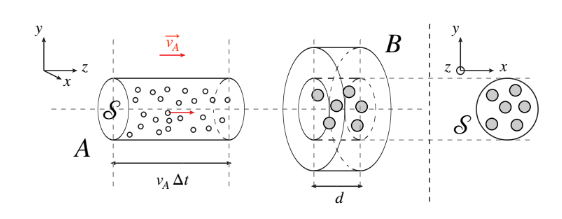
\includegraphics[scale=0.5]{ch4SezioneUrto/Scattering}
        \caption{Figura rubata dalle mitiche dispende del professor Kado}
\end{figure}
\newpage
Indichiamo il flusso di particelle che attraversazione la sezione trasversale S del bersaglio:
\begin{align*}
    \Phi = \dot{N_{p}}\frac{1}{S}
\end{align*}
Mentre il numero di particelle $N_{b}$ viste dai proiettili è :
\begin{align*}
    N_{b} = n_{b}Sd
\end{align*}
possiamo dire quindi con certezza che il rate di interazioni che avvengono è proporzionale 
a questi due termini : 
\begin{align*}
        \dot{N_{r}} &\propto \Phi N_{b} \\
                    &\propto \dot{N_{p}}n_{b}d
\end{align*}
ed è quì che entra in gioco la \textbf{sezione d'urto}, ossiamo come \textbf{coefficiente di  \\ proporzionalità}
\begin{align*}
    &\dot{N_{r}} = \sigma_{r}\dot{N_{p}}n_{b}d \\
    &\sigma_{r} = \frac{\dot{N_{r}}}{\dot{N_{r}}n_{b}d} \\
    &[\sigma_{r}] = \text{lunghezza}^{2} = \text{superficie}
\end{align*}
Indichiamo con \textbf{Luminosità istantanea} : 
\begin{align*}
    &L_{ist} = \dot{N_{p}}n_{b}d \\
    &[L_{ist}] = cm^{-2}s^{-1} 
\end{align*}
La luminosità è utile quando si lavora in processi di scattering fra due fasci di particelle
poichè si può scrivere in funzione del numero di particelle : 
\begin{align*}
    L = \frac{N_{a}N_{b}}{s}f_{rev} \tag*{$f_{rev}$ è la frequenza di rivoluzione}
\end{align*}
\subsection{Interpretazione geometrica}
La probabilità che una reazione avvenga è data da $\frac{\dot{N_{r}}}{\dot{N_{p}}}$, in un 
visione semplificata possiamo esprimere la probabilità come rapporto fra la superficie del 
proiettile e quella del bersaglio:
\begin{align*}
P = \frac{S_{r}}{S} = \frac{S_{eff}N_{b}}{S} \tag*{S = superficie flusso} \\ \tag*{$S_{eff}$ = superficie singolo bersaglio}
\end{align*}
si ottiene, ricordando la definizione di $N_{b}$ : 
\begin{align*}
        &\frac{\dot{N_{r}}}{\dot{N_{p}}} = S_{eff}n_{b}d \\
        &\sigma = S_{eff}
\end{align*}
tale interazione però non è del tutto esatta, infatti se prendiamo come bersaglio un protone 
e lo bombardiamo con diverse particelle si ottiene le sezioni d'urto sono differenti seppur
la $S_{eff}$ è sempre la stessa.
\newpage
\section{Una visione più sperimentale}
In un eseperimento quello che si fa è far interagire due fasci di particelle A e B, si pone 
un rivelatore in un certo punto dello spazio e si misurano il numero di interazioni per unità di tempo
che avvengono, da cosa dipende questo numero ? 
\begin{itemize}
        \item dinamica dell'interazione, ossia la sezione d'urto ;
        \item natura del bersaglio : tanto più alte sono le particelle bersaglio tanto 
                più alto è questo numero;
        \item flusso di particelle.
\end{itemize}
Il numero di interazioni, come abbiamo visto, si calcola:
\begin{align*}
    \dot{N_{r}} = \sigma_{r}\dot{N_{p}}n_{b}d
\end{align*}
\subsection{Come calcoliamo $n_{b}$}
La risposta è semplice : 
\begin{align*}
        n_{b} = \rho\frac{N_{A}}{A}
\end{align*}
dove $N_{A}$ è il numero di Avogradro e A è il numero di massa del materiale.
\subsection{Come calcoliamo $\dot{N_{p}}$}
Ovviamente non possiamo metterci a contare le particelle che passano per unità di tempo 
ma quello che si può fare è, conoscendo la carice delle particelle proiettile, ricavarci la 
corrente infatti : 
\begin{align*}
    i = \dv{q}{t} = q\dot{N_{p}}
\end{align*}
Facciamo un esempio : si ha un fascio di particelle $\alpha$ con carica i = 15 nA, calcoliamo 
$\dot{N_{p}}$. \\
\begin{align*}
        i = \dv{q_{\alpha}}{t} = q_{\alpha}\dot{N_{p}}
\end{align*}
ma, trattandosi di particelle $\alpha$, ossia nuclei di Elio, $q_{\alpha} = 2\abs{e}$ 
dove $\abs{e} = 1,6\times10^{-19}C$, ora dobbiamo trasformare i nA in $\frac{C}{s}$ : 
\begin{align*}
    1nA = 1\times10^{-9}A = 1\times10^{-9}\frac{C}{s}
\end{align*}
ed il gioco è fatto.
\newpage

\chapter{L'esperimento di Rutherford}
\section{Thomson vs Rutherford : chi ha ragione?}
Nei primi anni del 900 vi erano due modelli atomici : 
\begin{itemize}
        \item Il \textbf{modello di Thomson} per il quale l'atomo e schematizzato come una sfera
                con densità di carica uniforme, sostanzialmente le cariche positive e 
                negative erano distribuite uniformemente.
        \item il \textbf{modello di Rutherford} l'atomo era costituito da un nucleo puntiforme
                carico positivamente al centro e le cariche negative che gli orbitavano attorno.
\end{itemize}
Nel caso del modello di Thomson il campo elettrico dovuto dalle cariche, per il teorema di 
Gauss è dato da:
\begin{figure}[!h]
    \centering
    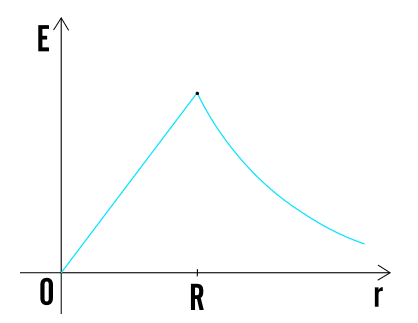
\includegraphics[scale=0.5]{ch5Ratherford/CampoE}
\end{figure}

Per capire come una particelle varia la direzione della quantità di moto, dobbiamo integrare
nel tempo la forza dovuta dal campo elettrico, integrale molto difficile, ciò che possiamo fare però è fare una maggiorazione poichè a noi interessa
la massima deflessione che la particella può subire.\\
$F_{max}$ per $r=R$ è:
\begin{align*}
    F_{max} = \frac{Ze\rho R}{3\epsilon_{0}}
\end{align*}
Essa si collega alla deflessione subita dalla particella dalla seguente:
\begin{align*}
        \theta_{max} = \frac{\Delta P}{P_{i}} = \frac{F_{max}\Delta t_{max}}{mv_{0}}
\end{align*}
Considerando il mezzo come una lamina d'oro e energia della particella di circa 5MeV si 
ottiene che la massima deflessione è :
\begin{align*}
    \theta_{max} \sim 3\cross10^{-4}rad
\end{align*}
Nello strato di oro che considereremo per l'esperimento di Rutherford si hanno circa 2000 atomi, 
essendo le deflessioni completamente casuali, considerando il processo come un Random Walk :
\begin{align*}
    \theta_{f} = \sqrt{2000}\theta_{max} \sim 1,3\cross10^{-2}rad
\end{align*}
Viene fuori che l'angolo massimo di deflessione che ci aspettiamo nel caso di uno scattering 
di una particella carica con un atomo descritto dal modello di Thomson è minuscolo, circa 
1 grado
\section{L'esperimento di Rutherford nella pratica}
Rutherford propose un modello atomico nel quale tutte le cariche positive sono concentrate 
in un piccolo volume al centro dell'atomo e le cariche negative orbitavano attorno ad esso.
L'esperimento che fece per provare ciò consisteva nel colpire tali atomi con particelle 
$\alpha$ le quali, entrando nel volume dell'atomo non sentiranno l'influenza del campo elettrico 
degli elettroni ( che per il teorema di Gauss è nullo ).
L'interazione fra le particelle $\alpha$ e il nucleo sarà trattato con metodi di meccanica 
classica e schematizzato come segue.
\begin{figure}[!h]
    \centering
    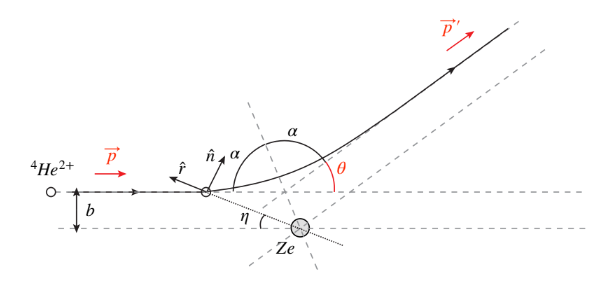
\includegraphics[scale=0.5]{ch5Ratherford/Rutherford}
    \caption{Tratiettoria della particella $\alpha$ deviata dal potenziale coulombiano del nucleo}
\end{figure}

dove : 
\begin{itemize}
        \item b = prametro di impatto; 
        \item $\theta$ = angolo di deflessione;
        \item \textit{z}e = carica particella $\alpha$; 
        \item Ze = nucleo bersaglio.
\end{itemize}
Ciò che vogliamo trovare è la relazione che intercorre fra il parametro di impatto e l'angolo
di diffusione, il fatto che trattiamo tale problema con metodi classici è molto importante 
perchè rende il problema \textbf{completamente deterministico}. \\
\begin{tcolorbox}[colback=red!5!white,colframe=red!50!black,title=ATTENZIONE !]
Perchè possiamo trattare il problema con metodi classici e non relativistici ? \\
In quegli anni non esistevano gli acceleratori di particelle, l'unica fonte erano quindi le radiazioni
che però producono proiettili con energia cinetica $T \sim 5MeV$ molto più piccola della massa della 
particella $\alpha$ che invece si aggira sui 4 GeV
\end{tcolorbox}
\newpage
La particella $\alpha$ subirà una forza repulsiva diretta radialmente :
\begin{align*}
    \va{F} = \frac{\textit{z}Ze^2}{4\pi \epsilon_{0}r^2}\vu{r}
\end{align*}
\begin{tcolorbox}[colback=red!5!white,colframe=red!50!black,title=ATTENZIONE !]
Il fatto che la forza sia centrale è molto importante poichè ci dice che la velocità non 
cambia se non in direzione, possiamo quindi applicare la conservazione del momento quantità 
di moto !
\end{tcolorbox}
Applichiamo la conservazione del momento quantità di moto : 
\begin{align*}
        \va{L} &= m_{\alpha}r^2\dv{\beta}{t} \\ 
        \va{L_{i}} &= m_{\alpha}bv_{0} 
\end{align*}
eguagliando si ottiene : 
\begin{align*}
    \frac{1}{r^2} = \frac{1}{bv_{0}}\dv{\beta}{t}
\end{align*}
Scriviamo ora l'equazione del moto \textbf{lungo l'asse y} : 
\begin{align*}
        m_{\alpha}\dv{v_{y}}{t} &= \frac{\textit{z}Ze^2}{4\pi\epsilon_{0}r^2}\sin{\beta} \\
        m_{\alpha}\dv{v_{y}}{t} &= \frac{\textit{z}Ze^2}{4\pi\epsilon_{0}bv_{0}}\sin{\beta}\dv{\beta}{t}
\end{align*}
Considerando due istanti A(t = -$\infty$) e B(t = $\infty$) : 
\begin{align*}
    v_{y}(A) = 0  & \quad  v_{y}(B) = v_{0}\sin{\theta} \\
    \beta(A) = 0  & \quad  \beta(B) = \pi - \theta 
\end{align*}
otteniamo : 
\begin{align*}
        \int_{0}^{v_{0}\sin{\theta}}\dd{v_{y}} = \frac{\textit{z}Ze^2}{4\pi\epsilon_{0}bv_{0}}\int_{0}^{\pi - \theta}\sin{\beta}\dd{\beta}
\end{align*}
finalmente arriviamo al risultato che volevamo ottenere all'inizio : 
\begin{align*}
        &v_{0}\sin{\theta} = \frac{\textit{z}Ze^2}{4\pi\epsilon_{0}bv_{0}}\qty[-\cos{\pi - \theta} + 1] \\[1em]
        &b = \frac{\textit{z}Ze^2}{4\pi\epsilon_{0}v_{0}^2}\frac{1 + \cos{\theta}}{\sin{\theta}} 
\end{align*}
\newpage
\begin{tcolorbox}[colback=red!5!white,colframe=red!50!black,title=ATTENZIONE !]
\begin{align*}
        b = \frac{\textit{z}Ze^2}{4\pi\epsilon_{0}bv_{0}}\cot{\frac{\theta}{2}}
\end{align*}
\end{tcolorbox}
\section{La sezione d'urto differenziale}
In un esperimento non si conosce il parametro di impatto della particella, non si può quindi
dato un determinato valore di b a quale valore di $\theta$ corrisponde, ma qualcosa possiamo fare ossia 
ricavarci la distribuzione di probabilità del parametro b considerando che possa essere distribuito 
lungo un anello centrato all'intorno della posizione del bersaglio.
\begin{figure}[!h]
    \centering
    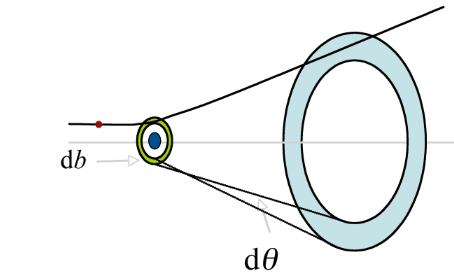
\includegraphics[scale=0.8]{ch5Ratherford/distribuzioneB}
\end{figure}

\begin{align*}
    &P(b)\dd{b} = \frac{2\pi b\dd{b}}{\pi R^2} \\[1em]
    &b = k\frac{1}{2}\cot{\frac{\theta}{2}} \quad \dd{b} = \frac{k}{2}\frac{\dd{\theta}}{2}\frac{1}{\sin^2{\theta/2}} \\[1em]
    &P(\Omega)\dd{\Omega} = \frac{\textit{z}Ze^2}{4\pi\epsilon_{0}bv_{0}}\frac{\dd{\Omega}}{16\sin^4{\theta/2}}\frac{1}{R^2\pi}
\end{align*}

$P(\Theta)$ non è altro che la probabilità dell'angolo soldo, essa è tanto più alta quando l'angolo di diffusione è basso, 
ma, ricordandoci che la sezione d'urto non è altro che la probabilità di un processo allora : 
\begin{align*}
        \dv{\sigma}{\Omega} = \frac{\textit{z}Ze^2}{4\pi\epsilon_{0}bv_{0}}\frac{1}{16\sin^4{\theta/2}}
\end{align*}

\chapter{Interazione radiazione-materia}
In questo capitolo ci occuperemo dell'interazione delle particelle con la materia, verrà diviso in tre sezioni : 
\begin{itemize}
        \item interazione di particelle cariche;
        \item interazione di fotoni; 
        \item interazione di neutroni.
\end{itemize}
\section{Interazione di particelle cariche con la materia}
Immaginiamo una particella con carica $\textit{z}e$ e massa m che attraversa un materiale di lunghezza $\dd{x}$ composto da atomi con numero di massa A e densità $\rho$
come in figura.
Ci chiadiamo quanto sia l'energia che perde la particella nell'attraversare il tratto $\dd{x}$ : 
\begin{align*}
    \frac{\dd{E}}{\dd{x}}
\end{align*}
\subsection{Perdita di energia per ionizzazione : la formula di Bohr}
Durante la derivazione della formula di Rutherford abbiamo assunto che se la particella ha un'interazione con il nucleo dell'atomo, la particella non perde 
energia siccome il nucleo ha una massa molto maggiore ma, così facendo, stiamo trascurando la possibilità di trasferire energia agli elettroni che è ciò che 
andremo a trattare in questa sezione.\\
\begin{figure}[!h]
    \centering
    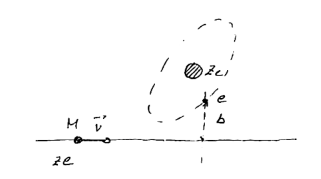
\includegraphics[scale=0.5]{ch6InterazioneMateria/BohrInterazione}
\end{figure}
\newpage
Dobbiamo calcolare l'energia cinetica ceduta all'elettrone ossia : 
\begin{align*}
        T_{e} = \frac{\Delta P_{e}^2}{2m_{e}}
\end{align*}
Per calcolare $\Delta P_{e}$ cambiamo sistema di riferimento in quello della particella dove quest'ultima è ferma e l'elettrone gli va incontro 
\begin{figure}[!h]
    \centering
    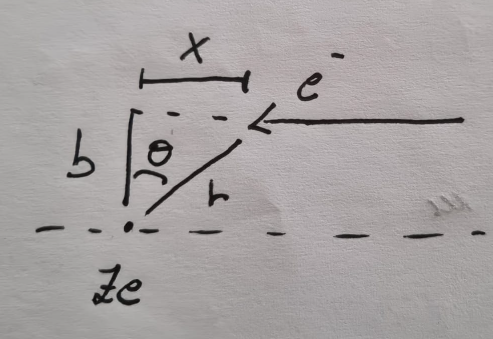
\includegraphics[scale=0.5]{ch6InterazioneMateria/CambioRiferimento}
\end{figure}

In una approssimazione non relativistica quindi possiamo vedere il tutto come un elettrone che passa nel campo culombiano di una particella con
carica $\textit{z}e$, attratto quindi da una forza : 
\begin{align*}
    F = \frac{\textit{z}e^2}{4\pi\epsilon_{0}}\frac{1}{r^2}
\end{align*}
possiamo dunque calcolare la quantità : 
\begin{align*}
        \Delta P_{e} &= \frac{\textit{z}e^2}{4\pi\epsilon_{0}}\int^{t}_{0}\frac{1}{r^2}\dd{t} \\
                     &= \frac{\textit{z}e^2}{4\pi\epsilon_{0}}\int^{\infty}_{-\infty}\frac{1}{r^2}\frac{\dd{x}}{v} \\
        \dd{t} &\rightarrow \frac{\dd{x}}{v} \tag*{Poichè v costante}
\end{align*}
Scomponiamo nelle due componenti considerando che $r = x^2 + b^2$ e che $(\Delta P)_{\parallel} = \Delta P\sin{\theta}$, $(\Delta P)_{\perp} = \Delta P\cos{\theta}$
otteniamo : 
\begin{align*}
        &(\Delta P)_{\parallel} =  \frac{\textit{z}e^2}{4\pi\epsilon_{0}v}\int\frac{1}{x^2 + b^2}\sin{\theta}\dd{x} = 0 \\
        &(\Delta P)_{\perp} =  \frac{\textit{z}e^2}{4\pi\epsilon_{0}v}\int\frac{1}{x^2 + b^2}\cos{\theta}\dd{x}
\end{align*}
\newpage
il secondo integrale lo calcoliamo sapendo che : 
\begin{align*}
        &\cos^2{\theta} = \frac{b^2}{x^2 + b^2} \\
        &\dd{x} = \frac{b}{\cos^2{\theta}}\dd{\theta}
\end{align*}
si ottiene : 
\begin{align*}
        (\Delta P)_{\perp} &=  \frac{\textit{z}e^2}{4\pi\epsilon_{0}vb}\int^{\frac{\pi}{2}}_{-\frac{\pi}{2}}\cos{\theta}\dd{\theta} \\
                           &= 2\frac{\textit{z}e^2}{4\pi\epsilon_{0}vb} \\
                           &= \frac{\textit{z}e^2}{4\pi\epsilon_{0}vb^2}\frac{2b}{v}
\end{align*}
\begin{tcolorbox}[colback=red!5!white,colframe=red!50!black,title=ATTENZIONE !]
nella formula sopra bisogna dire che : 
\begin{itemize}
        \item $ \frac{\textit{z}e^2}{4\pi\epsilon_{0}vb^2}$ = forza trasversale; 
        \item $\frac{2b}{v}$ = scattering time ; 
        \item abbiamo assunto che l'elettrone si muova su una linea dritta, ciò va bene se assumiamo che la velocità della particella sia molto maggiore 
                della velocità di orbita dell'elettrone.
\end{itemize}
\end{tcolorbox}

Troviamo così, nel caso non relativistico, l'energia persa : 
\begin{align*}
        \Delta T_{e} &= \frac{\Delta P_{e}^2}{2m_{e}} \\ 
                     &=\frac{2\textit{z}^2e^4}{m_{e}v^2b^2(4\pi\epsilon_{0})^2} 
\end{align*}
Introducendo $\beta = \frac{v}{c}$ e il raggio classico dell'elettrone $r_{e} = \frac{e^2}{4\pi\epsilon_{0}m_{e}c^2}$
\begin{align*}
        \Delta T_{e} &=  \frac{2\textit{z}^2e^4}{m_{e}c^2\beta^2b^2(4\pi\epsilon_{0})^2} \\
                     &= \frac{2\textit{z}^2m_{e}c^2}{\beta^2b^2}\qty[\frac{e^2}{4\pi\epsilon_{0}m_{e}c^2}]^2 \\
                     &= \frac{2\textit{z}^2m_{e}c^2}{\beta^2b^2}r_{e}^2
\end{align*}
\newpage
Dal punto di vista della particella incidente, il materiale che incontra può essere visto come un " fascio "
di elettroni distribuiti su una corona cilindrica a distanza comprese fra b e b + $\dd{b}$ come in figura
\begin{figure}[!h]
    \centering
    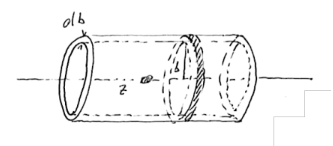
\includegraphics[scale=0.5]{ch6InterazioneMateria/DistribuzioneElettroni}
\end{figure}
Se $n_{e}$ è la densità degli elettroni nel materiale allora il numero di elettroni che 
la particella incontra in un tratto $\dd{x}$ è dato da : 
\begin{align*}
    \dd{N} = n_{e}V = n_{e}2\pi b\dd{b}\dd{x}
\end{align*}
Il valore dell'elemento di energia persa in un tratto infinitesimale $\dd{x}$ e dato il parametro di impatto 
\begin{align*}
    \frac{\dd[2]{E}}{\dd{x}\dd{b}} = n_{e}r_{e}^2m_{e}c^2\frac{4\pi}{b}\frac{z^2}{\beta^2}
\end{align*}
otteniamo quindi quello che volevamo cercare ossia l'energia persa per unità di lunghezza
\begin{align*}
        \frac{\dd{E}}{\dd{x}} &= n_{e}r_{e}^2m_{e}c^2\frac{4\pi z^2}{\beta^2}\int_{b_{min}}^{b_{max}}\frac{1}{b}\dd{b} \\[1em]
                              &= n_{e}r_{e}^2m_{e}c^2\frac{4\pi z^2}{\beta^2}\ln{\frac{b_{max}}{b_{min}}}
\end{align*}
Quello che bisogna fare ora è stimare $b_{min}$ e $b_{max}$.\\
\begin{itemize}
        \item Dato il principio di indeterminazione 
                \begin{align*}
                    \Delta p\Delta x = \hbar
                \end{align*}
            Se consideriamo $\Delta p$ come il momento dell'elettrone $p_{e}=m_{e}\gamma\beta c$
            otteniamo la risoluzione spaziale minima 
            \begin{align*}
                b_{min} = \frac{\hbar}{m_{e}\gamma\beta c}
            \end{align*}
    \item Come abbiamo detto, avendo considerato la traiettoria dell'elettrone sostanzialmente dritta 
        implica che lo scattering time definito sopra come $b/v$ deve essere relativamente piccolo rispetto al 
        tempo di rivoluzione dell'elettrone attorno all'atomo:
        \begin{align*}
            \gamma T_{e} = \gamma/w_{e}
        \end{align*}
        dove il fattore $\gamma$ tiene in considerazione della dilatazione del tempo.
        Come conseguenza si ottiene: 
        \begin{align*}
            b_{max} = \frac{\beta\gamma c}{w_{e}}
        \end{align*}
\end{itemize}
Otteniamo quindi la \textbf{formula di Bohr} : 
\begin{align*}
        \frac{\dd{E}}{\dd{x}} = 4\pi\rho N_{A}\frac{Z}{A}r_{e}^2m_{e}c^2\frac{z^2}{\beta^2}\ln{\frac{m_{e}c^2\beta^2\gamma^2}{\hbar w_{e}}}
\end{align*}
\subsection{Interpretazione della formula di Bohr}
La formula di Bohr dipende debolmente dal mezzo infatti, a parte costanti, la sua dipendenza 
è nel termine $Z/a$ che è nella stragrande maggioranza dei casi $\sim 1/2$. \\
Il termine più influente riguardante il mezzo è $\rho$, per tale motivo, per rendere la formula indipendente dal mezzo 
bersaglio di definisce : 
\begin{align*}
        \frac{1}{\rho}\frac{\dd{E}}{\dd{x}} &= 4\pi N_{A}\frac{Z}{A}r_{e}^2m_{e}c^2\frac{z^2}{\beta^2}\ln{\frac{m_{e}c^2\beta^2\gamma^2}{\hbar w_{e}}} \\[1em]
        \qty[\frac{1}{\rho}\frac{\dd{E}}{\dd{x}}] &= \frac{MeVcm^2}{g} 
\end{align*}
La dipendenza della particella è invece nel termine $Z^2/\beta^2$, ci sono due cose da dire: 
\begin{itemize}
        \item $Z^2$ : a parità di tutto, uno ione carbonio ( Z=6 ) scala 36 volte di più di un protone;
        \item la dipendenza da $\beta$ è scomoda poichè $0<\beta<1$ e per particelle relativistiche $\beta \sim 1$, conviene 
                esprimere dunque il grafico in funzione di $\beta\gamma$
\end{itemize}
\begin{figure*}[h!]
        \centering
        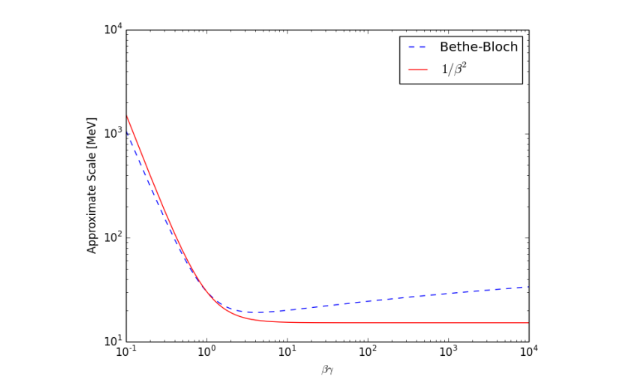
\includegraphics[scale=0.5]{ch6InterazioneMateria/BohrGrafico}
\end{figure*}

Per piccoli valori di energia, il termine dominante va come $1/\beta^2$ ad indicare che particelle lente perdono molta 
più energia rispetto a particelle più veloci.
A confronto con il semplice andamento di $1/\beta^2$ notiamo che vi è una piccola risalita nella perdita di energia, 
risalita dovuta al termine logaritmico, dovuto all'incremento del campo elettrico \\ " visto " dalla particella a velocità 
molto elevate, tale comportamento è denominato \textbf{risalita relativistica}.
\newpage
\subsection{La formula di Bethe-Bloch}
Una formula più generale, valida anche in casi realativistici, è quella di Bethe-Bloch:
\begin{align*}
    \frac{1}{\rho}\frac{\dd{E}}{\dd{x}} = C\frac{Z}{A}\frac{z^2}{\beta^2}\qty(\ln{\frac{2m_{e}c^2\beta^2\gamma^2}{I}}-\beta^2-\frac{\delta(\gamma)}{2})
\end{align*}
dove : 
\begin{itemize}
        \item abbiamo raccolto tutti le costanti $C=4\pi r_{e}^2c^2m_{e}N_{A} \simeq 0.307\frac{MeVcm^2}{g}$;
        \item la perdita di energia ha un minimo chiamato MIP \textit{ minimal-ionising particles } che 
                corrisponde a un $\beta\gamma \simeq 3$
\end{itemize}
\begin{figure}[!h]
    \centering
    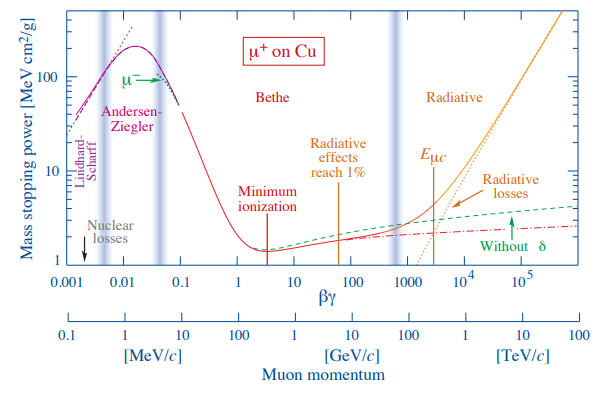
\includegraphics[scale=0.5]{ch6InterazioneMateria/BetheCompleta}
\end{figure}
Di questo grafico, che esprime la perdita di energia per ionizzazione su scale inferiori a quelle del momento del muone, 
la parte centrale fra le due bande grigie è ben descritta dalla formula di Bethe-Bloch.
\begin{itemize}
        \item Nella regione di sinistra, con valori di $\beta\gamma$ molto piccoli, il modello descritto fino ad ora non è 
                più valido, entrano in gioco effetti legati al fatto che la velocità del proiettile è paragonabile
                alla velocità di orbita degli elettroni;
        \item per grandi valori di $\beta\gamma$ il nostro modello non è valido, la perdita di energia è dovuta all'irraggiamento, 
                effetto di cui parleremo più avanti.
\end{itemize}
\begin{tcolorbox}[colback=red!5!white,colframe=red!50!black,title=ATTENZIONE !]
        La formula di Bethe-Bloch è un'espressione della perdita \textbf{media} di energia, siccome i processi di interazione
        fra particella e atomo è un processo stocastico, dobbiamo allora considerare anche la perdita di energia come casuale.
\end{tcolorbox}
\newpage
Per materiali spessi, il teorema del limite centrale ci assicura che le fluttuazioni siano gaussiane, questo non vale 
per materiali sottili, che seguiranno invece la distribuzione di Landau con code verso destra, ossia che vi sia un piccola 
probabilità di avere grandi perdite di energia.
\begin{figure}[!h]
    \centering
    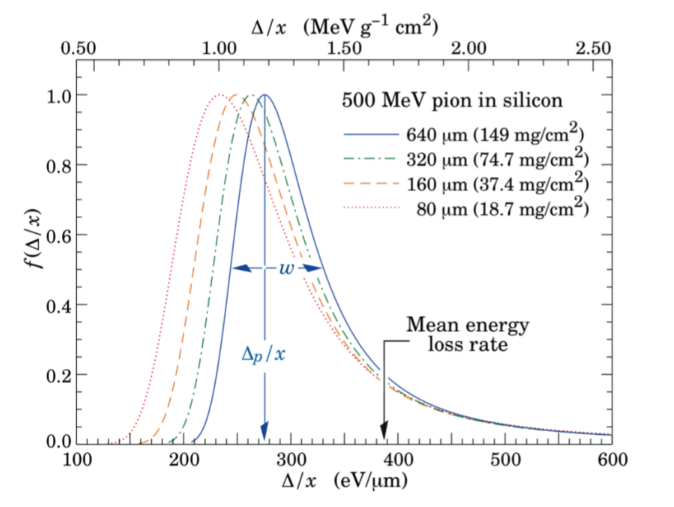
\includegraphics[scale=0.5]{ch6InterazioneMateria/Landau}
\end{figure}
\subsection{Il percorso residuo}
Si definisce come il percorso medio che compie una particella prima di perdere tutta la sue energia, quello che succede è che, 
perdendo energia, si risale la curva dell
\subsection{Effetto Cherenkov}
Quando una particella carica attraversa un mezzo polarizza gli atomi del materiale i quali rilasciano
radiazioni sotto forma di onde sferiche che hanno una velocità ( in un mezzo non dispersivo ) di :
\begin{align*}
        v_{g} = \frac{c}{n} \tag*{n è indice di rifrazione}
\end{align*}
\newpage
Quando la particella ha una velocità superiore a quella della luce nel mezzo vi è una convoluzione di queste onde sferiche che formano
un fronte d'onda, una luce quindi emessa ad un certo angolo $\theta_{c}$.
\begin{figure}[!h]
    \centering
    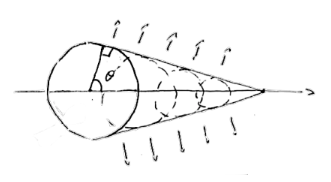
\includegraphics[scale=0.8]{ch6InterazioneMateria/Cherenkov}
\end{figure}

L'angolo di emissione è dato dalla relazione: 
\begin{align*}
        c\beta\cos{\theta_{c}} &= \frac{c}{n} \\[1em]
    \cos{\theta_{c}} &= \frac{1}{\beta n}
\end{align*}
L'equivalente meccanico di questo fenomeno è il boom supersonico.
\subsection{La perdita di energia per irraggiamento}
Fin'ora non abbiamo considerato cosa succede se la particella proiettile fosse un elettrone, 
in questo caso la formula di Bethe-Bloch deve essere modificata poichè bisogna tener conto 
dell'identità tra proiettile e bersaglio.\\
Un effetto importante è l'emissione di radiazioni elettromagnetiche provocata dall'accelerazione
dovuta all'urto elastico con il nucleo.
Tale perdita di energia per irraggiamento è data dalla :
\begin{align*}
        \frac{\dd{E}}{\dd{x}} &= 4r_{e}^2\alpha\frac{N_{a}Z^2\rho}{A}\ln{(183Z^{-1/3})}E \\[1em]
                              &\sim \frac{E}{X_{0}}
\end{align*}
a tale contributo va sommato quello di ionizzazione.\\
Bisogna notare che tale perdita per irraggiamento è lineare in E ciò comporta che, per un 
certo valore di E, tale contributo supera quello dovuto dalla ionizzazione.
Tale valore critico è detto appunto \textbf{energia critica} e vale:
\begin{align*}
    E_{c} = \frac{800}{Z+1.2}MeV
\end{align*}
La costante $X_{0}$ è detta \textbf{lunghezza di radiazione}, definita come la distanza alla
quale l'energia dell'elettrone si riduce di un fattore 1/e.
\section{L'interazione fotoni-materia}
Anche in questo caso bisogna suddividere l'interazione del fotone con gli elettroni, nel caso
venire assorbito (Effetto fotoelettrico) o cedere un po di energia (Effetto Compton), oppure
con il nucleo (produzione di coppie).
\subsection{Effetto fotoelettrico}
L'interazione avviene fra il fotone e un elettrone che è ancora legato al nucleo, la reazione 
completa è la seguente:
\begin{align*}
    \gamma+X\rightarrow X^{+}+e^{-}
\end{align*}
Affinchè tale reazione possa avvenire deve essere rispettata la conservazione dell'energia:
\begin{align*}
    &E_{\gamma}+m_{X}=m_{X^{+}}+m_{e}+T_{e}\\
    &E_{\gamma} = m_{X^{+}}+m_{e}-m_{X}+T_{e}\\
    &E_{\gamma} = E_{ion}+T_{e}
\end{align*}
Ciò comporta che una parte dell'energia del fotone è necessaria per ionizzare ( o anche solo eccitarlo ),
l'altra per dare energia cinetica all'elettrone, questo spiega la struttura a dente del grafico
della sezione d'urto del processo, picchi che sono in corrispondenza di energie del fotone 
compatibili con i livelli energetici degli shell dell'atomo.
\begin{figure}[!h]
    \centering
    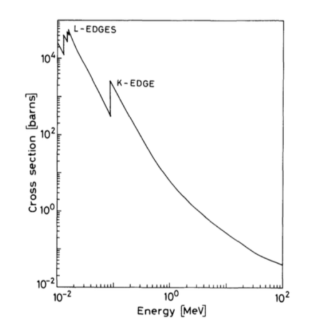
\includegraphics[scale=0.5]{ch6InterazioneMateria/Fotoelettrico}
\end{figure}
\newpage
\subsection{Effetto Compton}
L'energia del fotone è molto più alta di quella di ionizzazione, possiamo considerare dunque l'elettrone
come fosse, a questi livelli di energia domina l'effetto Compton rispetto al fotoelettrico.
Lo scattering fra il fotone e l'elettrone è di tipo elastico dato dalla seguente reazione:
\begin{align*}
    \gamma+e^{-} \rightarrow \gamma+e^{-}
\end{align*}
\begin{figure}[!h]
    \centering
    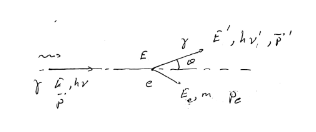
\includegraphics[scale=0.7]{ch6InterazioneMateria/Compton}
\end{figure}

utilizziamo la conservazione dell'energia e dell'impulso:
\begin{align*}
    &E+m_{e} = E^{\prime}+E_{e}\\
    &\va{p}=\va{p^{\prime}}+\va{p_{e}}
\end{align*}
dalla seconda si ottiene:
\begin{align*}
    &\va{p_{e}} =\va{p}-\va{p^{\prime}} \\
    &p_{e}^2 = p^2+p^{\prime2}-2pp^{\prime}\cos{\theta}\\
    &p_{e}^2 = E_{e}^2-m_{e}^2
\end{align*}
ricavando l'energia dell'elettrone dalla conservazione dell'energia e facendo un po di calcoli
che non riporterò si ottiene:
\begin{align*}
    E^{\prime} = \frac{m_{e}E}{m_{e}+E-E\cos{\theta}}
\end{align*}
Interessante esprimere le energie del fotone in termini di lunghezza d'onda:
\begin{align*}
    &E=\frac{hc}{\lambda} & E^{\prime} = \frac{hc}{\lambda^{\prime}}
\end{align*}
si ottiene (pure in questo caso ometto i semplici calcoli):
\begin{align*}
    \lambda^{\prime} = \lambda +\frac{h}{m_{e}c}(1-\cos{\theta})
\end{align*}
dove troviamo la \textbf{lunghezza d'onda di Compton}:
\begin{align*}
    \lambda_{c} = \frac{h}{m_{e}c}\simeq 2,4\cross10^{-12}m
\end{align*}
\subsection{Produzione di coppia}
Processo nel quale il fotone viene assorbito dal nucleo producendo una coppia elettrone-positrone 
secondo il processo:
\begin{align*}
    \gamma + X \rightarrow X + e^{-} + e^{+}
\end{align*}
Affinchè il processo avvenga deve essere :
\begin{align*}
    E_{\gamma} > 2m_{e}c^2
\end{align*}
\section{Neutrone-materia}
Da fare, è facilissimo non mi va ora
\newpage
\chapter{I decadimenti radioattivi}


\chapter{Fusione e fissione nucleare}
\section{Fissione nucleare}
Negli anni '30 i ragazzi di via Palisperna fanno esperimenti in cui si accorgono che, bombardando con 
neutroni terminci, si possa indurre radioattività: senza accorgersene avevano scoperto il 
fenomeno della fissione indotta.\\
Solo successivamente, in Germania, si accorsero che bombardando Uranio si ottenevano atomi
con A e Z di circa la metà.\\
Prendiamo dunque la reazione:
\begin{align*}
    X^{A}_{Z} \rightarrow Y^{A/2}_{Z/2} + Y^{A/2}_{Z/2}
\end{align*}
calcoliamoci il Q:
\begin{align*}
        Q &= M_{X}-2M_{y}\\
          &= -B_{x}+2B_{y}\\
          &=-7.5A + 2\frac{A}{2}8.5\\
          &\sim 200MeV \tag*{Per atomi pesanti}
\end{align*}
dove abbamo scritto la massa di un nucleo come la somma dei nucleoni meno l'energia di ionizzazione B.\\
Notiamo che Q è molto grande, ad atomi pesanti dunque conviene dividersi in atomi più leggeri,
i 200MeV di differenza finirà in energia cinetica dei due atomi.
\subsection{Cosa succede all'atomo durante la fissione}
Possiamo immaginare che il nucleo, durante il processo, cominci ad allungarsi ellitticamente
\newpage
\begin{figure}[!h]
    \centering
    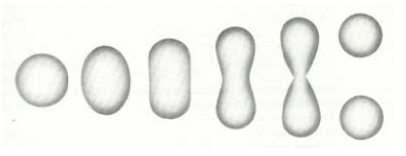
\includegraphics[scale=0.5]{ch6InterazioneMateria/NucleoFissione}
    \caption{Nucleo che si sta separando}
\end{figure}

All'interno del nucleo abbiamo visto (modello a goccia) che vi sono termini di interazione fra i 
nucleoni, in particolare:
\begin{itemize}
        \item Termine di superficie: è il termine che rema contro il legame nucleare, esso 
                in questa separazione sta aumentando:
        \item Termine culombiano : termine, aiuta il legame del nucleo, che dipende dalla distanza fra i protoni, durante la 
                separazione la distanza fra essi aumenta, diminuendo di conseguenza tale termine.
\end{itemize}
Manca l'immagine ma vediamo cosa succede con più esattezza ai termini sopra:
\begin{align*}
    &b_{1}A^{2/3}\rightarrow b_{1}A^{2/3}(1-\frac{2}{5}\epsilon^2)\\[1em]
    &b_{2}\frac{Z(Z-1)}{A^{1/3}}\rightarrow b_{2}\frac{Z(Z-1)}{A^{1/3}}(1-\frac{\epsilon^2}{5})
\end{align*}
Si nota come il primo termine (quello superficiale) aumenta e il secondo (culombiano) diminuisce.\\
A questo punto dobbiamo confrontare le masse dei nuclei nella forma sferica e in quella ellissoidale e
vedere quando la seconda è privilegiata rispetta la prima.
\begin{align*}
        M(sfera)-M(ellissoide) &= -B_{sf}+B_{elis} \\
                               &= -b_{1}A^{2/3}+b_{1}A^{2/3}(1-\frac{2}{5}\epsilon^2)-b_{2}\frac{Z(Z-1)}{A^{1/3}}+b_{2}\frac{Z(Z-1)}{A^{1/3}}(1-\frac{\epsilon^2}{5}
\end{align*}
Questo non è altro che il celeberrimo Q value che abbiamo visto anche nei decadimenti, 
andiamo a vedere quando esso è maggiore o minore di 0:
\begin{align*}
    2b_{1}\frac{Z^2}{A^{1/3}}>< b_{2}\frac{Z^2}{A^{1/3}}\rightarrow \frac{2b_{1}}{b_{2}}><\frac{Z^2}{A}
\end{align*}
Sapendo che $2b_{1}/b_{2}\sim50$ si deduce che non è assolutamente scontato che un atomo faccia
fissione spontaneamente ma tanto più è grande $Z^2/A$ più è probabile che succeda. 
\newpage
\subsection{Fissione nucleare indotta}
Per spiegare la fissione indotta ci concentriamo sui nuclei $U^{235}_{92}$ e $U^{238}_{92}$, 
seppur la concentrazione del primo sia nettamente inferiore questo ha una importanza straordinaria
e vediamo ora il perchè.
Per avere fissione indotta si ha un neutrone che colpisce il nucleo producendo 2 prodotti di fissione e
2 o 3 neutroni.
\begin{tcolorbox}[colback=red!5!white,colframe=red!50!black,title=ATTENZIONE !]
I prodotti di fissione non sono definiti univocamente, la distribuzione di fissione ha 2 picchi.
\end{tcolorbox}
A livello energetico quello che succede è questo : quando un U 235 viene colpito da un neutrone 
termino si crea un nucleo $U^{236*}$ eccitato, ossia con energia poco superiore a quella del
$U^{236}$.
Ci calcoliamo l'energia di eccitamento:
\begin{align*}
    &M(U^{236*}) = M(U^{235})+n \\
    &E_{ecc} = M(U^{236*})-M(U^{236}) \simeq 6,54MeV 
\end{align*}
Se consideriamo l'energia di soglia per la quale avviene la fissione $E_{sogl}\sim 6MeV$ notiamo che in 
questo caso avviene la fissione.
Studiamo ora il caso del $U^{238}$, il ragionamento è esatamente lo stesso ma si ottiene:
\begin{align*}
    E_{ecc} = M(U^{239*})-M(U^{239}) \sim 4,8MeV
\end{align*}
Il fatto è che U 238 è pari-pari e per il nuclei pari-pari l'energia di legame è più alta,
ciò implica che il neutrone termico non riesce a dare abbastanza energia per eccitare il nucleo e 
dare via alla fissione.

\appendix
\chapter{Costanti e Unità di misura}
\section{Unità di misura}
\begin{itemize}
        \item $1 \unit{\ampere} = 1 \unit{\coulomb\per\second\squared}$
        \item $1 b = 10^{-24} \unit{\centi\metre\squared}$
        \item $1 \unit{\electronvolt} = $
\end{itemize}

\end{document}
